\documentclass{article}
\usepackage{malmacros}
\begin{document}

\section{MLP MNIST}

\subsection{Qa Using a Keras MLP on the MNIST-data'}
In this section the steps from the Keras moon exercises are redone with the MNIST data set. With some help/inspiration from the examples in the exercises from Googles Colab quickstart guides, that was refered to by a fellow student. The link to guides are in the code.
\\ \\
First bit of preparing the data, with help from the colab guide. 
To fit the dimensions and the handle the mnist data in general we have to flatten the data.

\begin{pyminted}
# With inspiration from the quickstart guide at: 
#https://colab.research.google.com/github/tensorflow/docs/blob/master/site/en/r2/tutorials/quickstart/beginner.ipynb

#Prepare the data:
from keras.datasets import mnist

(X_train, y_train), (X_test, y_test) = mnist.load_data()
X_train, X_test = X_train/255.0, X_test/255.0 # Convert to floats

y_train_binary = to_categorical(y_train)
y_test_binary = to_categorical(y_test)

# y = y_train
assert y_train.ndim==1
assert y_train_binary.ndim==2
assert y_test_binary.ndim ==2


model = Sequential()
model.add(Flatten(input_shape=(28,28)))
model.add(Dense(128, activation='relu'))
model.add(Dropout(0.2))
model.add(Dense(10, activation='sigmoid')) # try softmax as well

optimizer = SGD(lr=0.1, momentum=0.9, nesterov=True)
model.compile(loss='categorical_crossentropy', 
              optimizer=optimizer, 
              metrics=['categorical_accuracy', 'mean_squared_error', 'mean_absolute_error'])

print("Ok")

\end{pyminted}

\noindent
 And then training the model afterwards. This lead to a fairly short training time of 11.8 seconds.
 
\begin{pyminted}
# Now to train the data:
# Train
VERBOSE     = 0
EPOCHS      = 5

from time import time

start = time()
history = model.fit(X_train, y_train_binary, validation_data=(X_test, y_test_binary), epochs=EPOCHS, verbose=VERBOSE)
t = time()-start

print(f"OK, training time={t:0.1f}")
\end{pyminted}

\noindent
And then the output of the data. Again using the SGD Optimizer like the first time with the Keras Moon data. But this time attempting to tune it a little bit by changing the first activation layer to \textbf{"relu"} and the second one to \textbf{"sigmoid"}, as they gave the best results in the last Keras Moon exercise. Figure\ref{fig:keras-mnist-a}.

\begin{figure}[H]
  \centering
    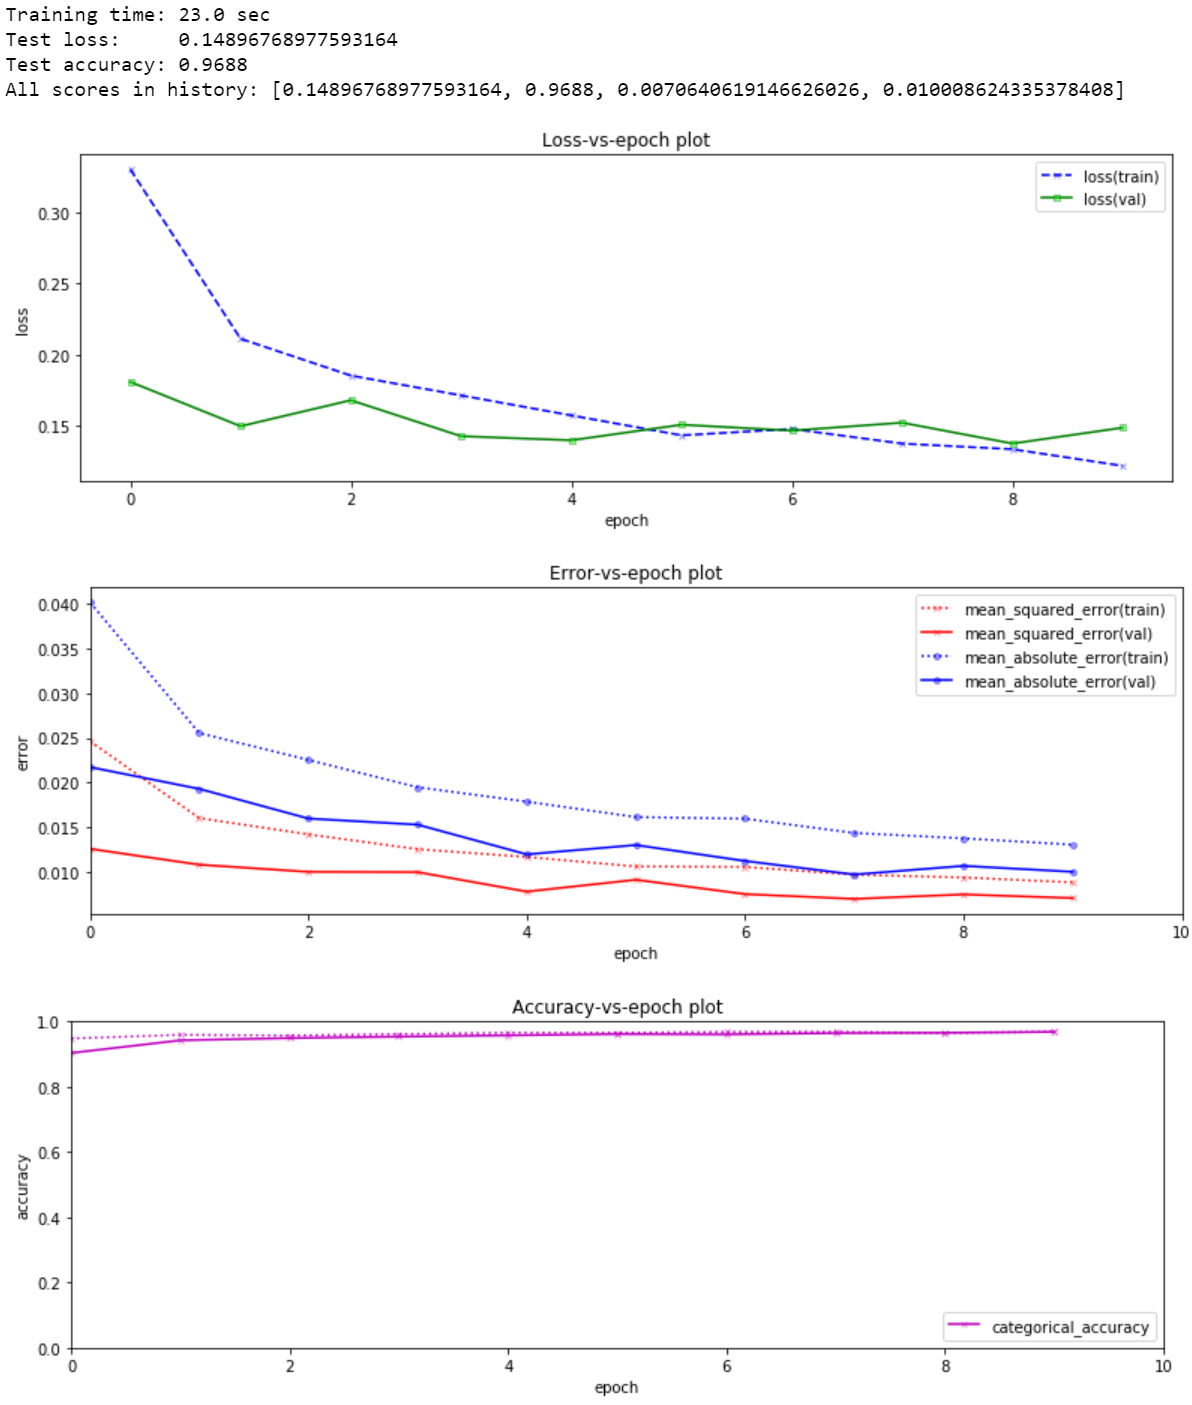
\includegraphics[width=0.8\textwidth]{keras-mnist-a}
    \caption{Output from Keras moon Qa, using the Adam optimizer.}
    \label{fig:keras-mnist-a}
\end{figure}

\subsection{Qb Repeat Grp10's Go at the Search Quest}
As it would be quite the task to "reverse engineer" our methods of setting up a GridSearch and doing the exhaustive searches for hyper paramethers but this time with keras, which is a taks in itself since they don't exactly make it easy, as the 2 libaries do most things differently. So instead we experiemented with other examples of setting up DNN, using some documented examples from Keras.io.
\\ \\
To try something different and to better accommodate for the MNIST data set being a visual data set, as it consist of 70000 images of hind-written numbers. A model was setup to use a \textbf{CNN}, \textit{Convolutional Neural Network}, also sometimes known as ConvNet. Its a type of neural network that is tailored for image recogniction and typical computer vision tasks, and its design is inspired by the biological visual cortex, the deeper explantion can be found here: \href{http://libccv.org/doc/doc-convnet/}{}. 
\\ \\
In this first snippet the data preparation for the deep convolution network is  shown. Setup with the inspiration from the example from keras.io and our own methods learned from previous exercises, the url is in the first comment of the snippet. The important difference to note here is how the data set is handled this time. All the images with the digits are setup with image rows and columns and using the Keras-backend to help us with some image formatting channels.


\begin{pyminted}
from __future__ import print_function
import keras
from keras.layers import Conv2D, MaxPooling2D
from keras import backend as K

#Defining our batchsize.
batch_size = 128
# This is simply for use when calling to_categorial.
#Telling it that there are 10 categories, one for each digit (0-9).
num_classes = 10
EPOCHS = 12

# setting up the image rows and columns, this is new particular part, when training the CNN.
img_rows, img_cols = 28, 28

# loading in the data like before.
(X_train, y_train), (X_test, y_test) = mnist.load_data()

if K.image_data_format() == 'channels_first':
    X_train = X_train.reshape(X_train.shape[0], 1, img_rows, img_cols)
    X_test = X_test.reshape(X_test.shape[0], 1, img_rows, img_cols)
    input_shape = (1, img_rows, img_cols)
else:
    X_train = X_train.reshape(X_train.shape[0], img_rows, img_cols, 1)
    X_test = X_test.reshape(X_test.shape[0], img_rows, img_cols, 1)
    input_shape = (img_rows, img_cols, 1)

# Same as before we convert the data types to floats.
# here using the method from colabs instead of the longwinded one from keras.io.
X_train, X_test = X_train/255.0, X_test/255.0 # Convert to floats

# checking the shape of the data:
print('x_train shape:', X_train.shape)
print(X_train.shape[0], 'train samples')
print(X_test.shape[0], 'test samples')

# convert class vectors to binary class matrices
y_train = keras.utils.to_categorical(y_train, num_classes)
y_test = keras.utils.to_categorical(y_test, num_classes)
\end{pyminted}

\newpage
\noindent
Then setting up the the layers using the sequential method. We add layers an using Conv2D as it is a 2D dimentional deep convolutional neural network. First layer added is a input layer, with 32 neurons, and an activation layer of type relu. Then adding another convulutio adding another similar but with twice the neurons. So each of the previous one map to 2 new ones. Then a layer pooling the data. And after this a layer using dropout, to prevent overfitting. Then a layer to flatten the data to preserve the dimensional weight ordering. And after this another activation layer, again doubling the neurons (up to 128) and, then a dropout an then the last activation layer, which finishes with softwax activation function.

\begin{pyminted}
model = Sequential()
model.add(Conv2D(32, kernel_size=(3, 3),
                 activation='relu',
                 input_shape=input_shape))
model.add(Conv2D(64, (3, 3), activation='relu'))
model.add(MaxPooling2D(pool_size=(2, 2)))
model.add(Dropout(0.25))
model.add(Flatten())
model.add(Dense(128, activation='relu'))
model.add(Dropout(0.5))
model.add(Dense(num_classes, activation='softmax'))

optimizer=keras.optimizers.Adadelta() # a more robust version of AdaGrad which was presented to us in the book. 
model.compile(loss='categorical_crossentropy', 
              optimizer=optimizer, 
              metrics=['categorical_accuracy', 'mean_squared_error', 'mean_absolute_error'])


# Then fitting and training the model, choosing verbose = 1 while training to see the progress as we go.
start = time() # our timer as before
history = model.fit(X_train, y_train,
          batch_size=batch_size,
          epochs=EPOCHS,
          verbose=1,
          validation_data=(X_test, y_test))
t = time()-start

print(f"OK, training time={t:0.1f}")
\end{pyminted}

\noindent
Enabling the verbose the progress could be seen as it trains the model, a feature we discovered late and could have used earlier as somtimes the training of mnist could take a LOOONG time, and waiting not knowing wether it would fail or it was hanging.
A frustration that could have been avoided using this earlier. But for the output is chosen to be omitted here, to save space. The training time using the AU GPU-cluster, was a nice and short: 52.9 seconds. And because we had the progress running we could se that on the training set it was scoring 99.18 percent accuracy.

\begin{pyconsole}
Epoch 12/12
60000/60000 [==============================] - 4s 73us/step - loss: 0.0268 - categorical_accuracy: 0.9916 - mean_squared_error: 0.0013 - mean_absolute_error: 0.0026 - val_loss: 0.0292 - val_categorical_accuracy: 0.9911 - val_mean_squared_error: 0.0014 - val_mean_absolute_error: 0.0022
OK, training time=52.9
\end{pyconsole}

\noindent
Now to evaluate on the test set. And using our plot methods from earlier to see the result. The full output is shown in figure \ref{fig:keras-mnist-cnn-output}. 

\begin{figure}[H]
  \centering
    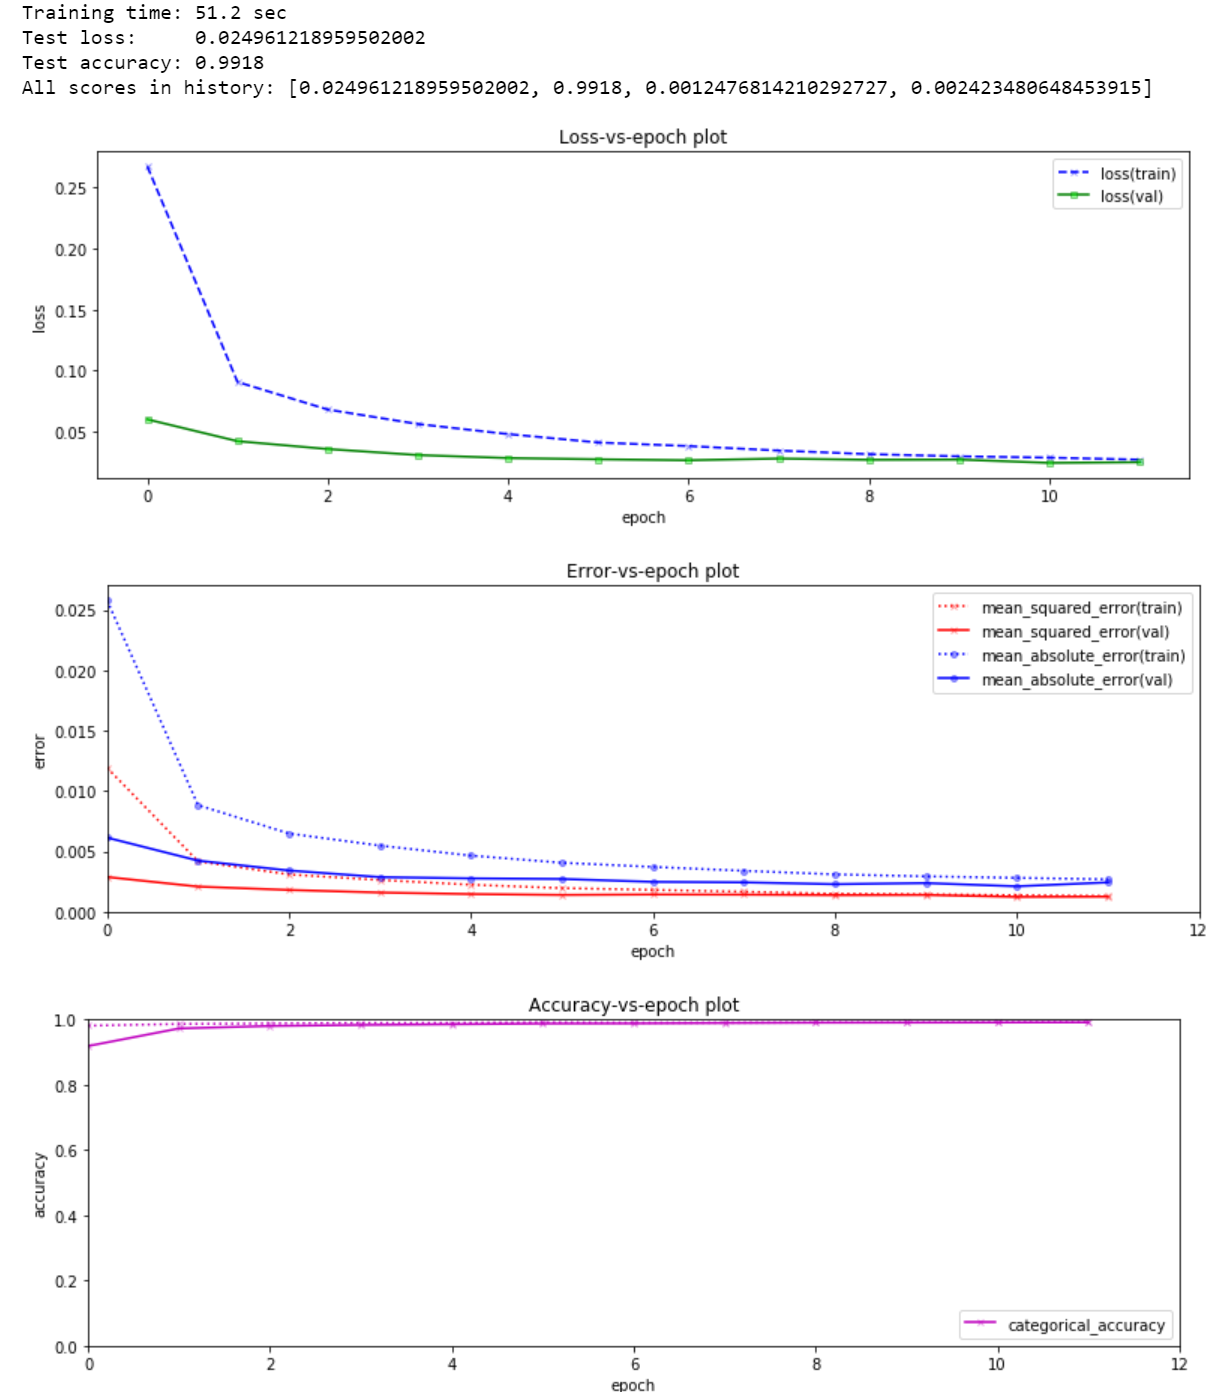
\includegraphics[width=0.8\textwidth]{keras-mnist-cnn-output}
    \caption{Full report output of the ConV Neural network using AdaDelta.}
    \label{fig:keras-mnist-cnn-output}
\end{figure}

\noindent
After this a try with the good old Nesterovs SGD optimizer \textbf{NAG} to see whether it could compare to the \textbf{AdaDelta} model. And it actually did quite well, almost the same score as the Adadelta with only about -0.02 percent deference, a shorter training time, and almost the same loss. Result shown in figure \ref{fig:keras-mnist-cnn-output-sgd}

\begin{figure}[H]
  \centering
    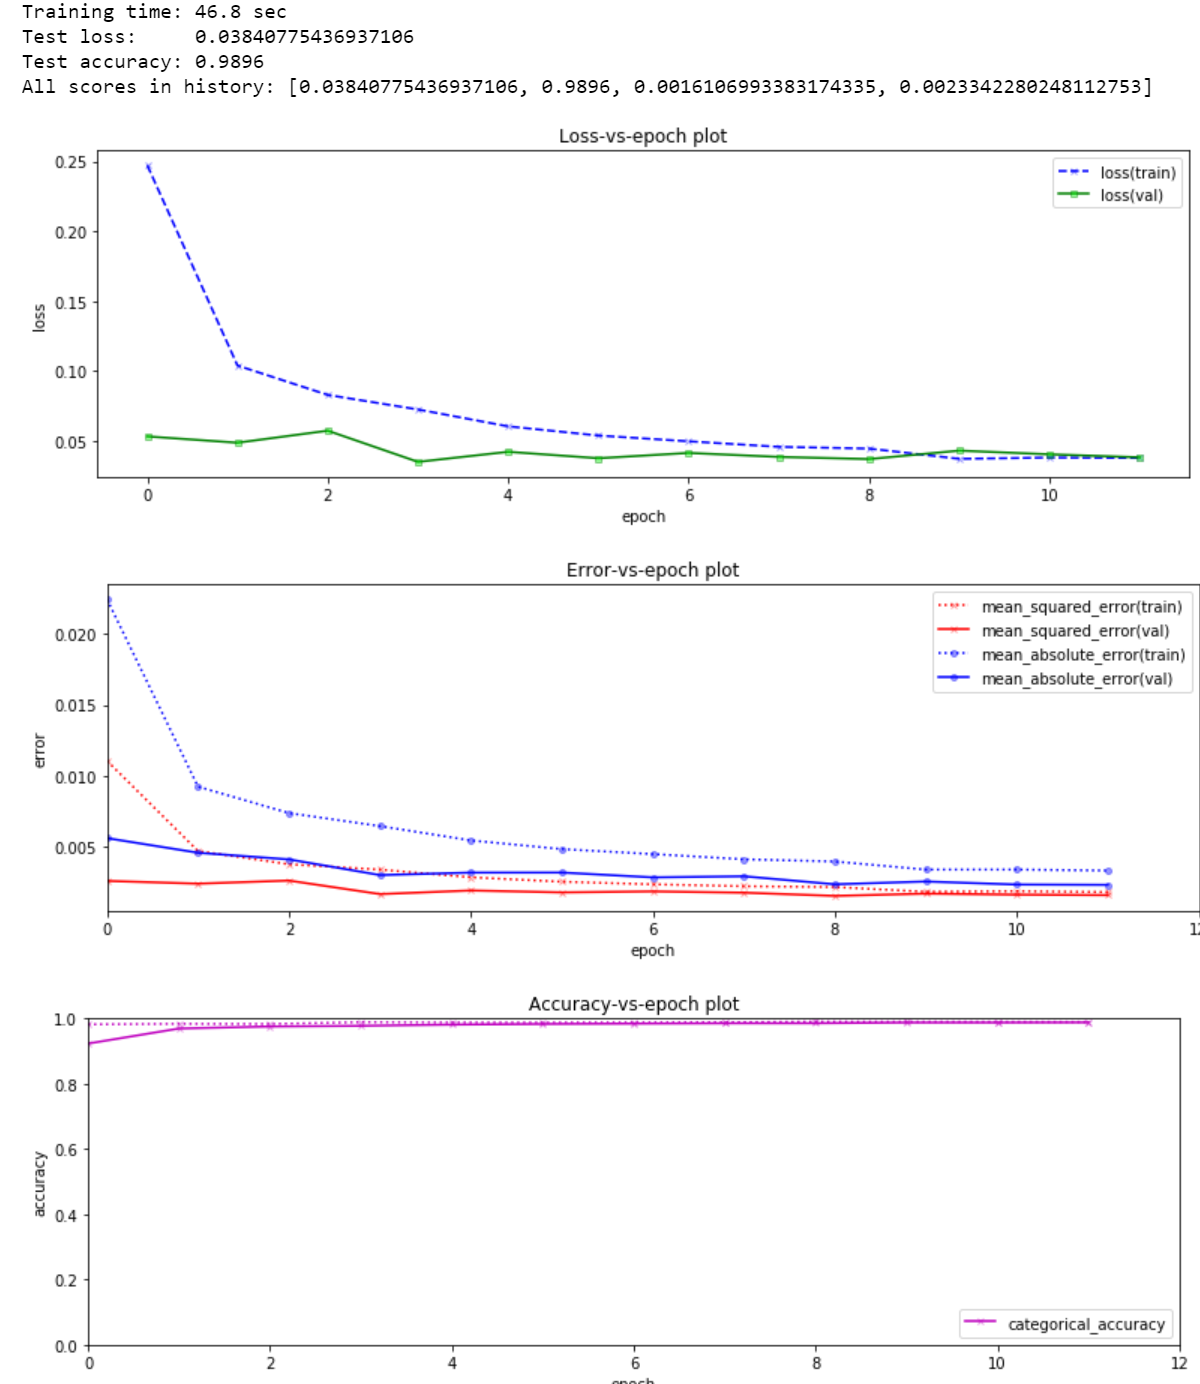
\includegraphics[width=0.8\textwidth]{keras-mnist-cnn-output-sgd}
    \caption{Full report output of the ConV Neural network using NAG.}
    \label{fig:keras-mnist-cnn-output-sgd}
\end{figure}

\noindent
But of course this test couldn't be concluded without also trying out the \textbf{Adam} optimizer.
Wow what a surprise, after hearing how well \textbf{Adam} just works out of the box, seeing how it did,
SO BAD, was unexpected. The result is shown in figure \ref{fig:keras-mnist-adam-bad}.

\begin{figure}[H]
  \centering
    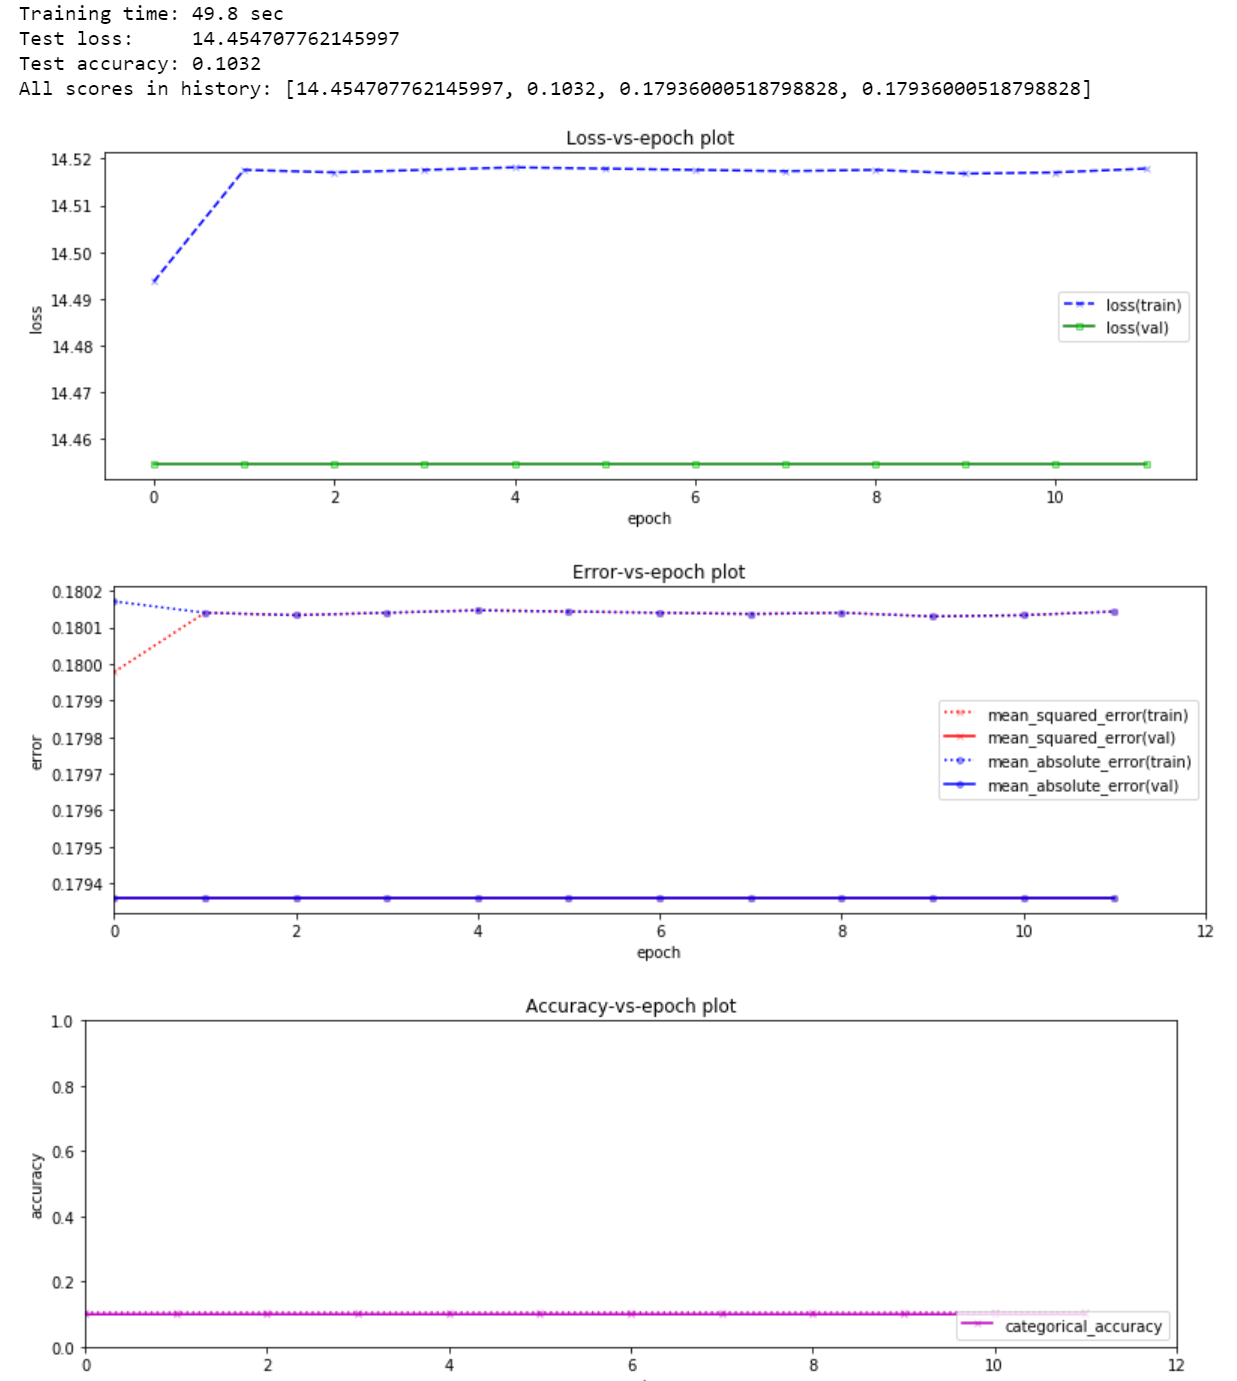
\includegraphics[width=0.8\textwidth]{keras-mnist-adam-bad}
    \caption{Full report output of the ConV Neural network using Adam.}
    \label{fig:keras-mnist-adam-bad}
\end{figure}

\noindent

But knowing it did well earlier, investegation was needed. So on to the documentation. It turned out that using the same initial learning rate of 0.1 for \textbf{Adam} as was set for us as an example in the earlier code, and that we had continued to use. Was the problem all along, setting the initial learning rate to 0.001 a factor 100 lower, which was found to be the default in the keras documentation, the result was a different story entirely as seen in figure \ref{fig:keras-mnist-adam-good}.
Comparing the 2 graphs its also visually clear to see now that the problem was the intial learning rate modifier \textbf{eta0} was far to high before, which resulted in badly under-fitting the data.

\begin{figure}[H]
  \centering
    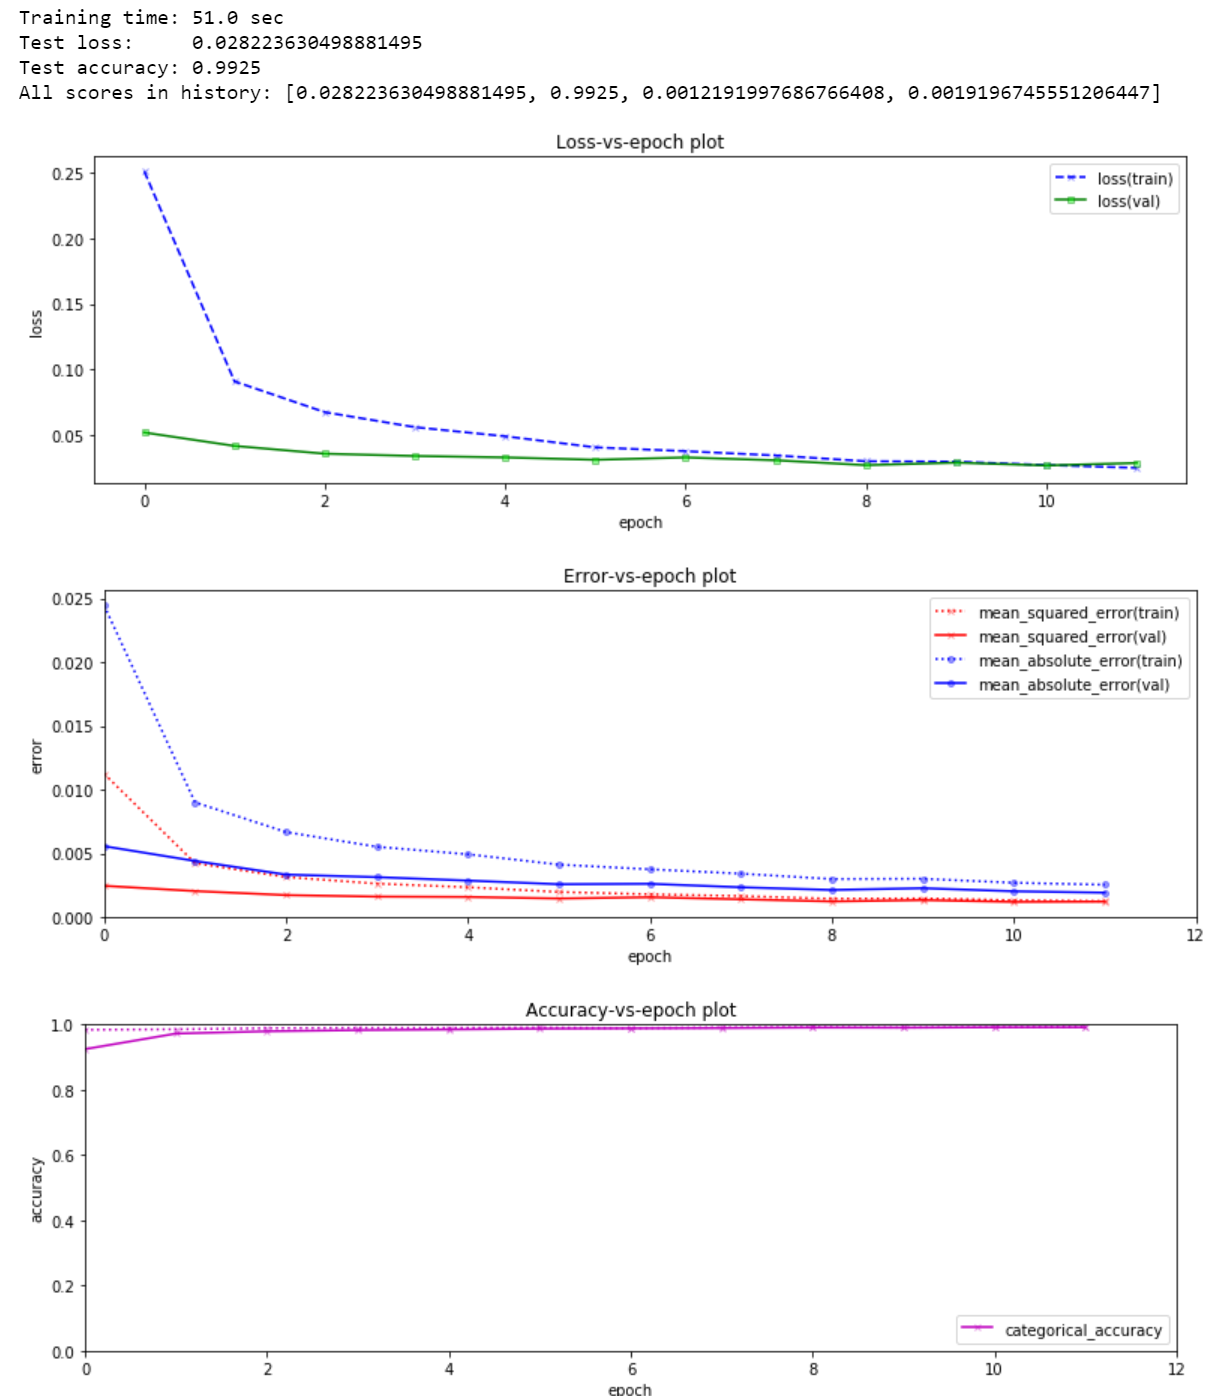
\includegraphics[width=0.8\textwidth]{keras-mnist-adam-good}
    \caption{Full report output of the ConV Neural network using Adam, now with a better result.}
    \label{fig:keras-mnist-adam-good}
\end{figure}

\end{document}

